Notre dictionnaire est donc un arbre n-aire. Nous allons d�tailler son
utilisation.\\
Un arbre n-aire peut �tre visualis� comme un arbre binaire mais o�
seulement un seul fils fait 'descendre' dans la profondeur de l'arbre, on
parle de fils et de fr�re. comme dans l'exemple qui suit:

\begin{figure}[h]
  \centering
  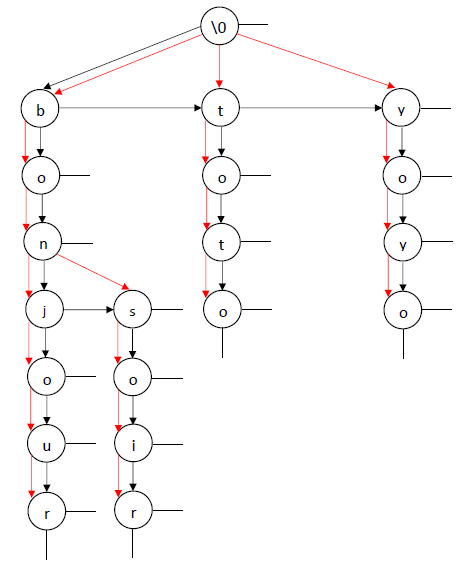
\includegraphics[width=10cm, height=12cm]{images/arbrenillustration.png}
  \caption{\label{�tiquette} Un exemple d'arbre n-aire}
\end{figure}

L�gende :
\begin{itemize}
\item[] Rouge : TAD Collection Arbre
\item[] Noir : Conception � l'aide d'un Arbre Binaire\\
\end{itemize}

Dans notre dictionnaire, la racine n'est pas utilis�e. Elle est ici pr�sente
car, par d�finition, la racine d'un arbre n-aire a un fr�re vide du
point de vue de la conception. Ici le 'a' est le fils de la racine et
le 't' est le fr�re de 'a'. L'int�r�t de cette repr�sentation est
qu'un mot devient un chemin de fils en fils et de fr�res en
fr�res. Pour savoir si un chemin est un mot valide, on rajoute un
champs � chaque noeud de notre arbre, une variable bool�enne
'motValide' par exemple. Sur la figure ci-dessus, si notre arbre
contient uniquement le mot 'yoyo', seulement le deuxi�me 'o' aura le
champ 'motValide' � VRAI car 'y', 'yo' et 'yoy' ne sont pas des mots
dans notre dictionnaire. Si on voulait ajouter le mot 'yoyos' il
suffirait d'ajouter le fils 's' au deuxi�me 'o' et d'avoir les champs
'motValide' � VRAI pour le deuxi�me 'o' et le 's'.